\documentclass{vldb}
\usepackage{algorithm}
\usepackage{algorithmic}
\usepackage[normalem]{ulem}
\usepackage{graphicx}
%\usepackage{times}
\usepackage{color}
\def\naive{na\"{\i}ve}
\newcommand{\todo}[1]{\textcolor{red}{{#1}}}
\newcommand{\eat}[1]{} % Used for multi-line commenting.
\newcommand{\topic}[1]{\par \smallskip \smallskip \noindent{\bf \uline{#1}}}
\newcommand{\topicnoul}[1]{\par \smallskip \smallskip \noindent{\bf {#1}}}
\newcommand{\fivespaces}{\ \ \ \ \ }
\newcommand{\INDSTATE}[1][1]{\STATE\hspace{#1\algorithmicindent}}
\usepackage[small]{caption}
\usepackage{url}
\DeclareCaptionType{copyrightbox}

\renewcommand\floatpagefraction{.9}
\renewcommand\topfraction{.9}
\renewcommand\bottomfraction{.9}
\renewcommand\textfraction{.1}
\setcounter{totalnumber}{50}
\setcounter{topnumber}{50}
\setcounter{bottomnumber}{50}


\newcounter{foo}
\newenvironment{myenumerate}{\begin{list}{\arabic{foo}.}{
	        \usecounter{foo}
			        \setlength{\leftmargin}{10pt}
					        \setlength{\topsep}{2pt}
							        \setlength{\itemsep}{1pt}
}}{ \end{list}}

\newenvironment{mylist}{\begin{list}{$\bullet$}
    {   \setlength{\itemsep}{2pt}
	        \setlength{\leftmargin}{10pt}
			        \setlength{\topsep}{2pt}}
					    }
						{\end{list}}

\def\sharedaffiliation{%
\end{tabular}
\begin{tabular}{c}}


% Writing author names..
% According to guidelines, there needs to be 3 per line.
% lines are separated using \and as shown below.
\author{
}

\date{}
\title{Large-Scale Cross-Validation using MapReduce}
\begin{document}
\maketitle

\begin{abstract}
With enormous amounts of data that is being generated at very scales, the
problem of efficiently learning patterns and features in the data has become
increasingly challenging. To this end, there have been significant efforts
toward building systems for solving such large-scale machine learning problems,
many of them using MapReduce. While existing systems provide support for
efficiently building machine learning models from data, they currently do not
consider two key issues in large-scale machine learning: First, evaluating the
quality of the learned models, i.e., estimating the {\em generalizability} of
the models to future (unseen) data sets and second, {\em model selection}, i.e.,
determining the best possible parameter values for a model (e.g., what is the
best $k$ value for $k$-means clustering). As with current approaches, we propose
to solve the above problems using cross-validation based algorithms.

%However, implementing large-scale cross-validation over MapReduce architectures
%is challenging owing to a number of reasons.
In this paper, we develop a {\em declarative system} for supporting
large-scale cross-validation (CV) over MapReduce clusters. We abstract the
common operations from CV e.g., partitioning, and formulate an algebra of
operators to support their execution. These operators can not only be
parameterized to support arbitrary machine learning models, but also provide
opportunities for plan-based optimization. We introduce a cost-based
optimization framework for choosing the best plans to evaluate, based on the
nature of the input and the resources available at hand. Our preliminary
experiments demonstrate the necessity of a declarative system for large-scale
CV, and the scalability of our proposed approaches.
\end{abstract}

\section{Introduction}
\label{sec:introduction}

Large-scale machine learning is emerging as a significant research problem in
recent times owing to the enormous amounts of data that is being generated at
increasing scales by a variety of data sources on the web. Examples include data
in the form of click logs, search logs, ad-impression logs, messages on social
networks, movie and product reviews and so on. Effectively mining and
understanding patterns from such data is critical for several applications e.g.,
spam detection, personalized search and advertising, recommender systems.
Furthermore, recent observations that accuracies of machine learned models can
be significantly improved by simply using larger amounts of (independent)
training data rather than using complex
models~\cite{DBLP:journals/expert/HalevyNP09} has fueled even more interest in
developing machine learning techniques that can scale to very large data sets.
Existing tools for large-scale machine learning include Matlab
and R~\cite{rr} and their parallel equivalents (Revolution-R~\cite{revolutionr}
and Parallel-Matlab~\cite{toolbox}). Lately, a number of systems have been
developed for scalably learning from large amounts of data based on
MapReduce~\cite{DBLP:conf/osdi/DeanG04}; examples include Apache
Mahout~\cite{mahout}, Google Prediction API~\cite{gapi},
SystemML~\cite{DBLP:conf/icde/TianK11}.  Further, there has been recent
literature~\cite{Low+al:uai10graphlab,DBLP:conf/nips/ChuKLYBNO06} for tailoring
algorithms for parallel machine learning. These systems have been used to solve
several real-world machine learning problems including classification, clustering,
collaborative filtering and probabilistic inference.
\eat{
Hence, there is a need for systems that can be used for machine
learning over very large-scale data. 
Existing tools for large-scale machine
learning include Matlab and R~\cite{rr} and their parallel equivalents
(Revolution-R~\cite{revolutionr} and Parallel-Matlab~\cite{toolbox}).  The
emergence of large-scale data processing systems such as
MapReduce~\cite{DBLP:conf/osdi/DeanG04} has led to a number of such efforts in
recent times. 
Chu et al.~\cite{DBLP:conf/nips/ChuKLYBNO06} abstract several
machine learning algorithms using the {\em summation form}, using which they
provide algorithms for parallelizing a large class of algorithms over MapReduce.
Apache Mahout~\cite{mahout} provides a suite of scalable machine learning
libraries for large-scale classification, clustering and collaborative filtering
problems. Google Prediction API~\cite{gapi} provides a simple API with pattern
matching and machine learning capabilities over Google's servers. Recently, Tian
et al.~\cite{DBLP:conf/icde/TianK11} proposed SystemML, which is a declarative
system for large-scale machine learning. SystemML provides a high level language
{\em DML} (similar to R), which can be used to write machine learning
abstractly. Internally, the system compiles and optimizes the code into a Hadoop
implementation.  The above systems have been deployed for solving large-scale
clustering and classification tasks, non-negative matrix factorization
problems~\cite{DBLP:conf/icde/TianK11}. While the current systems have been very
useful for solving a wide variety of machine learning problems, they currently
do not support the following critical tasks.
}
While the above systems make it easier to learn models from very large-scale
data, they currently do not support the following key tasks.

\begin{enumerate}
\item
First, the ability to {\em validate the quality of models} learned, i.e.,
estimate how well the model will perform on a future unseen dataset.
Overfitting~\cite{Kohavi95featuresubset} is a commonly observed
problem in machine learning that occurs when the learned model, which is only
supposed to learn features in the data, also learns noise. This typically occurs
when the model is too complex (far too many parameters) for the dataset. When a
model is overfit to the training data, its generalization is poor and it does
not work well with future data. Hence it is very important to validate the learned
models before deploying it for real world problems.

\item 
The second task is to estimate the best values for model parameters, commonly
known as the {\em model selection}
problem~\cite{Scheffer/Joachims/99a,DBLP:journals/bioinformatics/TroyanskayaCSBHTBA01}. 
\eat{Model selection is the
problem of selecting the right model and picking the right parameters for the
model.} Model selection is very critical to the accuracy of the learned models.
For example, consider a document clustering application that uses k-means
clustering. If we use a very small value for $k$, then multiple documents that
are not similar would end up in the same cluster, conversely if we choose a very
large value for $k$, then similar documents may end up in different clusers. 

\item
The
third task is {\em feature selection}, which is the problem of selecting
a subset of relevant features for building robust models. This problem is
critical in high dimensional datasets, which is commonly seen in web
data~\cite{DBLP:conf/icdm/MalikK08,Kriegel:2009:CHD:1497577.1497578} and significantly impacts the quality of classification
models~\cite{DBLP:journals/jmlr/GuyonE03}.
\end{enumerate}

\eat{\item {\em Learning complex models:} This is a class of classification algorithms
that build a set (or an ensemble) of classifiers that are usually more accurate
than any single classifier. Ensemble learning algorithms have been used recently
in the Netflix prize, almost every entry in the top-10 used some kind of
ensemble.}

All of the problems listed above are typically solved using {\em
cross-validation} (CV), which is a well established concept in machine learning.
Briefly, the cross-validation procedure involves creating multiple copies of the
dataset called {\em folds}, each of which has a training (held in) component and a test
(held out) component. The model to be validated is learned using the train component
and evaluated against the test component of each fold by measuring the error,
e.g., the number of mis-classifications or error in regression.
The average error across all the folds is used as a representative of the {\em
generalizability} of the learned model, i.e., how it performs
on future data sets. A large cross-validation error indicates overfitting
and the need for using simpler models. For solving the model-selection problem,
these errors are computed for different choices of the model/parameters and the
model with the smallest error is chosen.
While there exist other techniques such as AIC (Akaike information
criterion), BIC (Bayesian information criterion) and
VC-dimension~\cite{Blumer:1989:LVD:76359.76371,citeulike:849862}, CV is the
most popular method used in practice, since it can be applied in general to a
very large class of models.

Existing systems provide little or no support for general
cross-validation. While R and Matlab do provide built-in support for cross-validation,
it is usually limited to packages that implement specific algorithms such as
linear regression or classification. Consequently, the users are forced to develop their own
implementations for CV for various models, leading to limited usability,
sub-optimal approaches and constant re-invention of the wheel. 
In this work, we develop a system for providing support for generic
cross-validation of a large class of machine learning models, i.e., we want to
support cross-validation as a high level construct.
However, supporting large-scale generic CV is challenging due to a number of
reasons.
\begin{mylist}
\item First, most CV techniques are usually specific to each maching learning model.
Constructing a generic abstraction for all known methods of cross-validation, while
retaining the efficiency, is challenging.
\item Second, cross-validation algorithms are highly compute-intensive and
data-intensive. CV involves generating multiple copies of (potentially large) input data set.
Although sampling the data can mitigate these issues, it has been empirically
verified~\cite{journals/prl/IsakssonWGG08,journals/bioinformatics/Braga-NetoD04} for CV, that the
resulting error estimates are biased and not indicative of the generalizability of the
model.
\item Supporting generic CV requires sophisticated algorithms for fold
construction. For instance, constructing folds for bootstrap CV requires complex sampling algorithms
such as {\em sampling with replacement}, which has been shown to be non-trivial to
parallelize(Panda et al.~\cite{DBLP:journals/pvldb/PandaHBB09}) on shared-nothing MapReduce architectures.
\item Further, fold construction for unsupervised learning algorithms such as PCA, SVD and
NMF~\cite{DBLP:conf/nips/LeeS00} require novel matrix partitioning techniques
(holding out cells \& sub-matrices) that are challenging to implement for very
large matrices of the order of millions of rows and columns.

\eat{
Parallelizing sampling {\em with replacement} over MapReduce is
non-trivial as has been shown 
\item Fourth, supporting cross-validation using bootstrapping requires
scalably implementing novel sampling algorithms over distributed MapReduce
architectures. As described in Panda et al.
scalably parallelizing sampling with replacement over MapReduce is non-trivial
since it requires maintaining state in memory which is inefficient in
shared-nothing architectures.
}
\end{mylist}

\topic{Our approach}\\
In this paper, we augment the SystemML~\cite{DBLP:conf/icde/TianK11} system to support large-scale
cross-validation. SystemML is a declarative system for large-scale machine
learning currently being developed at IBM. It provides a {\em declarative} language,
called DML, which allows users to write machine learning code at a high-level of
abstraction. In SystemML, the user's DML code is compiled and optimized
into a  {\em dag} of MapReduce jobs. To implement generic cross-validation in SystemML, we develop a single general operator
for cross-validation that abstracts its core features (such as partitioning)
and which can be parameterized to instantiate different models. We provide
various implementations for each operator: we provide three
different implementations of the partitioning operator, each of which is
optimal under different data characteristics. Next we develop a novel cost-model
for determining the best possible plan for a given CV task. The research
contributions of our work are:

\begin{enumerate}
\item  We develop a generic abstraction that lets a user to apply CV to a large
class of machine learning models -- both supervised and unsupervised. To the
best of our knowledge, ours is the first system that has been developed for
cross-validating unsupervised models on very large matrices.

\item {\em Sampling as joins:} We develop techniques for efficiently executing
complex sampling algorithms over MapReduce using traditional database joins.

\item In addition to computing efficient plans, we develop
novel scheduling algorithms for executing the tasks, based on available
resources (e.g., disk space which is a bottleneck because of multiple copies
required).

\item {\em Cost model:} Developed a cost-model for different implementations of
the above operators and introduced a cost-based optimization framework for
executing these tasks, just as with relational query processing.

\end{enumerate}

\begin{figure*}
\hspace*{-0.1in}
\small
\centering
\begin{tabular}{ccc}
\begin{minipage}{3.0in}
%\fbox{
\begin{minipage}{3.0in}
\begin{algorithmic}
\STATE{V = {\bf readMM}(``V", {\bf rows}=1000, {\bf cols}=1000,}
\INDSTATE[12]{{\bf format}=``text");}
\STATE{W = {\bf Rand}({\bf rows}=1000, {\bf cols}=10, {\bf min}=0, {\bf max}=1);}
\STATE{H = {\bf Rand}({\bf rows}=1000, {\bf cols}=10, {\bf min}=0, {\bf max}=1);}
\STATE{max\_iterations = 20;}
\STATE{i = 0;}
\WHILE{(i $<$ max\_iterations)}
\STATE{H = H * (t(W) \%*\% V) / (t(W) \%*\% W \%*\% H);}
\STATE{W = W * (V \%*\% t(H)) / (W \%*\% H \%*\% t(H));}
\STATE{i = i+1; }
\ENDWHILE
\STATE{{\bf writeMM}(W, ``w.output", {\bf format}=``text");}
\STATE{{\bf writeMM}(H, ``w.output", {\bf format}=``text");}
\end{algorithmic}
\end{minipage}
%}
\end{minipage}
&
\begin{minipage}{1.75in}
\includegraphics[width=1.75in]{dml}
\end{minipage}
\hspace*{-0.1in}
&
\begin{minipage}{2in}
\includegraphics[width=2in]{nmfcv-illustration}
\end{minipage}\\
(a) DML code for NMF (non-negative matrix factorization)  & (b) SystemML
architecture & (c) $2\times2$ Gabriel holdouts
\end{tabular}
\caption{(a) High-level DML code for NMF is shown here. (b) The five layer
design for SystemML (c) Illustration of $2\times2$ Gabriel holdouts. In the
first step, the rows are columns are split into two groups. Subsequently, $4$
folds are constructed in which a given row and column group is held out and the
remaining data is held in.}
\label{fig:intro}
\end{figure*}


\section{Preliminaries}
\label{sec:background}
In this section, we provide background for the various concepts used throughout
the paper. We start with a discussion of SystemML. Following this, we provide a short
description of cross-validation and the most commonly used CV methods for both
supervised and unsupervised learning tasks.

\subsection{SystemML}
We illustrate the architecture of SystemML with an example. As mentioned
in Section~\ref{sec:introduction}, SystemML exposes a high level language --
DML, which allows a user to write machine learning code abstractly.
The system translates the DML code into a {\em dag} of MapReduce jobs over
a Hadoop cluster.
As an example, the implementation of {\em non-negative matrix
factorization}, a commonly used method for topic modeling and recommender
systems, is shown in Figure~\ref{fig:intro}(a). As shown in the figure, constructs in
DML include linear algebra operations such as matrix multiplications, looping
constructs (while), and conditioning
(if). SystemML is designed as a five layer system as shown in
Figure~\ref{fig:intro}(b). The DML code is transformed and optimized at each layer,
finally into a MapReduce dag which is scheduled/orchestrated by the Control system.
The {\em parser} performs static analysis over the code and
computes a {\em dag} of high level operations (HOPS dag). The {\em HOPS} layer
optimizes the dag (e.g., computes a good order for matrix multiplications) and
constructs a new dag over low-level operations. While high level operations
(HOPs) represent operations such as matrix multiplications over the data
matrices, low-level operations (LOPs) corresponds to operations over key-value
pairs (which constitute the data matrices). Finally, the LOPS layer
topologically sorts the lops dag and groups together the low-level operations
which can be executed in a single MapReduce job. The {\em control system} then
schedules the jobs over the Hadoop cluster. We refer the reader to Tian et
al.~\cite{DBLP:conf/icde/TianK11} for a more comprehensive discussion of
SystemML.

\subsection{Crossvalidation (CV)}
\label{sec:cvbackground}
Cross-validation is a technique for estimating the accuracy of a machine learned
model over a future (unseen) dataset. Widely used in supervised classification
problems, CV techniques compute an error for a given machine learned model,
which is indicative of its generalization performance. Cross-validation error is
computed by splitting the
given data set into a training (held in) and testing (held out) components. Such
a split is called as a {\em fold}. A model is learned over the training
component and the error is evaluated over the test
component. Typically, the error is averaged over multiple such folds to reduce bias. 
CV has been used for a number of problems such as preventing overfitting, model
selection, and feature selection. We now illustrate the most common methods used
for cross-validating both supervised and unsupervised models.

\topic{Supervised learning:}\\
The input dataset to a supervised learning problem is a set of data points
with known class labels. We visualize the data as a matrix with rows
corresponding to the data points and the columns corresponding to the
features. We assume that one of the columns corresponds to the class label.
There are a number of different ways of constructing folds, three of which are
illustrated next.

\begin{itemize}
\item \underline{\em k-fold:} In k-fold cross-validation, the input matrix is initially
split (row-wise) into $k$ groups. Following this, $k$ folds are constructed:
the $i^{th}$ fold is constructed by using the $i^{th}$ group as the
test component and the remaining $k-1$ groups as the train component. For each
fold, a model is learned over the training data and its error is evaluated over
the test data set. Finally, errors are averaged across the folds.
\item \underline{\em $\mu$-holdout:} In holdout cross-validation, a fraction ($\mu$) of the
input rows is held out and forms the test component. The remaining set of rows
form the train component and are used to train the model. Typically, the above
operation is repeated for a number of user-specified iterations. 
\item \underline{\em Bootstrap:} For Bootstrap cross-validation, we create the training
component by sampling the original dataset with replacement. The entire dataset
acts as the test component. As before, we construct as many folds are specified
by the user.
\end{itemize}

K-fold cross-validation ensures that every data point is part of exactly one
test component. Hence, we use every data point as a test component in some fold.
Holdout cross-validation allows us to construct small holdouts without
replicating the dataset too many times. For instance, if we want to holdout out
10\% of the data for testing, then using k-fold cross-validation requires us to
use k=10, which involves replicating the data set 10 times. Using holdout
cross-validation allows us to use 10\% of the data for testing using arbitrary
number of iterations. {\em Leave-one-out} cross-validation is essentially k-fold
cross-validation where $k$ is equal to the number of data points.  Leave-one-out
cross-validation is expensive and unsuitable for cross-validation over very
large-scale data. Bootstrap cross-validation is useful when the size of the
dataset is very small (since it replicates data points). Another commonly used
parameter in CV for supervised models is {\em stratified sampling}.  Consider a
spam detection task where we need to classify a given email as spam or not.
Suppose that in our training dataset, we have 80\% genuine emails and 20\% spam
emails. In that case, stratification allows each fold to have the same
percentage of spam and genuine emails in both the train and test components. We
describe how to support stratification in Section~\ref{sec:implementation}.

\topic{Unsupervised learning:}\\
It is not immediately obvious how to cross-validate unsupervised learning models
since the training data is not annotated with class labels. Indeed, there has
been very little prior work~\cite{wold,gabriel} on cross-validating unsupervised
models, much of it focusing on PCA (principal component analysis).
With increasing usage of unsupervised techniques such as NMF (for topic
modeling and recommender systems) and SVD (for dimensionality reductions) there have been
proposals~\cite{PerryO09,nips2010} for cross-validating unsupervised models.
Recently, Kanagal et al.~\cite{nips2010} demonstrate the connection
between matrix completion~\cite{CandesTao} and cross-validating unsupervised
models, resulting in many novel methods for cross-validation.
These techniques make use of the observation that unsupervised learning
algorithms essentially learn the {\em distribution} of the input data for
developing cross-validation algorithms for them. For example, a clustering
algorithm essentially learns the underlying distributions that generates the
given dataset. A topic modeling algorithm over
documents builds a generative model from which the document collection can be
generated. Hence, most of the proposed techniques holdout
portion of the data, build an unsupervised model over the held-in data and
either reconstruct the held-out data points using the learned model or measure the
likelihood that the held-out data points actually come from the learned model.
By measuring such errors (reconstruction or
perplexity~\cite{DBLP:journals/jmlr/BleiNJ03}), CV is used to estimate the parameters of the
model, i.e., number of useful principal components in SVD or the number of
topics in a topic model. Next, we describe two commonly used fold construction methodologies for
unsupervised models.

\begin{itemize}
\item \underline{\em $h\times l$ Gabriel holdout:} In this case, the rows of the matrix
are partitioned into $h$ row-groups and the columns of the matrix are
partitioned into $l$ column-groups. Following this, $hl$ folds are defined in
which a given row-group and a column-group is held-out and the remaining
components of the matrix are held-in. An illustration of Gabriel holdout for
$2\times 2$ is shown in Figure~\ref{fig:intro}(c). As shown in the figure, (for
Fold 1), a model is learned using matrices $B$, $C$ and $D$. Similarly, for Fold
2, $B$ is held out and the model is learned over matrices $A$, $C$ and $D$.
Owen \&
Perry~\cite{PerryO09} describe a methodology for reconstructing the held-out
matrix ($A$ in Fold 1) based on the entries in the held-in matrix ($B$, $C$ and
$D$ in Fold 1).
\item \underline{\em Wold holdout:} In this case, a fraction of cells in the matrix are
heldout, similar to $\mu$-holdouts. In recent work, Kanagal et
al.~\cite{nips2010} develop techniques for reconstructing the values of these
cells based on weighted NMF~\cite{DBLP:conf/icml/SrebroJ03}.
\end{itemize}

As illustrated above, supervised and unsupervised models use different
strategies for fold construction. Supervised models typically
holdout rows from the matrix since each row has a class label associated with
it and unsupervised models holdout cells or submatrices. 
\eat{In
the next section, we provide a unified abstraction for the various
cross-validation methodologies discussed here.}

\begin{figure}
\centering
\includegraphics[width=3.5in]{illustration}
\caption{The figure illustrates the four different steps involved in cross-validation
using two folds. In the first step, data is partitioned (and replicated) and
folds are constructed. In the second step, a model is learned over the train
component. Subsequently, the model is evaluated over the test component and the
errors are aggregated.}
\label{fig:illustration}
\end{figure}

\section{Cross-Validation Abstraction}
\label{sec:abstraction}
In this section, we provide a unified abstraction for the various
cross-validation strategies discussed in Section~\ref{sec:background} by
introducing the CV language construct. This supports generic cross-validation
for a large class of machine learning models.

\subsection{Cross-validation}
Cross-validation can be schematically described using four modules as
illustrated in Figure~\ref{fig:illustration}.
\begin{enumerate}
\item {\em partition:} Partitioning and replicating the dataset into {\em
folds}, where each fold has a training and a testing component. Note that the
training component may either be a single matrix or a set of matrices.
\item {\em cvtrain:} For each fold, train a model using the specified algorithm
over the training component of the fold.
\item {\em cvtest:} For each fold, evaluate the learned model using the testing
component of the fold and return the error.
\item {\em agg:} Finally, we aggregate the errors computed in
each fold, e.g., using either {\tt SUM} or {\tt AVG}.
\end{enumerate}

\topic{Language construct} \\
Based on the above abstraction, we introduce the following high-level construct
for generic cross-validation. \\
\begin{center}
\framebox[3.3in][c]{
\begin{minipage}[t]{3.2in}
{ {\bf crossval} $<$datasets$>$} \\
{ {\bf partition}}
{ ({\bf method}={\em `kfold'$|$`holdout'$|$`bootstrap'}}, \\
\hspace*{39pt}{ {\bf element}={\em `submatrix'$|$`row'$|$`cell'}}, \\
\hspace*{39pt}{ method specific parameters)} { {\bf as}  $<$outputs$>$}  \\
{ {\bf cvtrain} trainfunction($<$inputs$>$) {\bf as} $<$model output$>$} \\
{ {\bf cvtest} testfunction($<$inputs$>$) {\bf as} $<$error$>$} \\
{ {\bf aggregate}} { {\em `avg' $|$ `sum'}}
\end{minipage}
}
\end{center}

\begin{figure*}
\small

\hspace*{-0.10in}
\begin{tabular}{ccc}

\fbox{
\begin{minipage}{3.2in}
\begin{algorithmic}
\STATE{mydata = {\bf readMM}(``mydata", {\bf rows}=1000, {\bf cols} = 1000,}
\STATE{\hspace*{1in} \ \ {\bf nnzs} = 100000, {\bf format}="text");}
\STATE{numtopics = 1;}
\WHILE{(numtopics $<$ 20);}
\STATE{{\bf crossval} mydata}
\STATE{\hspace*{10pt} {\bf partition} ({\bf method} =`kfold', {\bf element}=`submatrix',}
\STATE{\hspace*{46pt} {\bf numRowGroups=2}, {\bf numColGroups}=2)}
\STATE{\hspace*{46pt} {\bf as} (A,B,C,D)}
\STATE{\hspace*{10pt} {\bf cvtrain} NMFCVTrain(B,C,D) {\bf as} (W,H)}
\STATE{\hspace*{10pt} {\bf cvtest} test(A,W,H) {\bf as} (error)}
\STATE{\hspace*{10pt} {\bf aggregate avg as} (output);}
\STATE{numtopics = numtopics + 1;}
\ENDWHILE
\end{algorithmic}
\end{minipage}}  &

\hspace*{-0.15in}
\begin{tabular}{c}

\fbox{
\begin{minipage}{2.4in}
\begin{algorithmic}
\STATE{{\bf function} NMFCVTrain(X, Y, Z) {\bf returns} (W, H) \{ }
\STATE{\hspace*{20pt}//Assume function (W,H) = NMF(X);}
\STATE{\hspace*{20pt}$(W_z,H_z)$ = NMF(Z);}
\STATE{\hspace*{20pt}$(W_z,H)$ = NMF(Y);}
\STATE{\hspace*{20pt}$(W,H_z)$ = NMF(X);}
\STATE{\} }
\end{algorithmic}
\end{minipage}
}  \\ \\
\fbox{
\begin{minipage}{2.3in}
\begin{algorithmic}
\STATE{{\bf function} test(A, W, H) {\bf returns} (error) \{ }
\STATE{\hspace*{20pt} diff = A - W * H;}
\STATE{\hspace*{20pt} error = norm(diff * diff);}
\STATE{\} }
\end{algorithmic}
\end{minipage}
}
\end{tabular} &
\hspace*{-0.25in}
\begin{minipage}{1.3in}
\includegraphics[width=1.3in]{combinations}
\end{minipage} \\
(a) CV construct for model-selection in NMF & (b) Test \& train routines called
in part (a) & (c) \\
\end{tabular} \\

\hspace*{-0.30in}
\begin{tabular}{cc}

\begin{tabular}{c}
\fbox{
\begin{minipage}{3.8in}
\begin{algorithmic}
\STATE{V = {\bf readMM}(``v.input", {\bf rows}=1000, {\bf cols}=1000, {\bf format}=``text") ;}
\STATE{y = {\bf readMM}(``y.input", {\bf rows}=1000, {\bf cols}=1, {\bf format}=``text") ;}
\STATE{{\bf crossval} (V,y)}
\STATE{\hspace*{10pt}{\bf partition} ({\bf method}=`holdout', {\bf element}=`row', {\bf
frac}=0.30)}
\STATE{\hspace*{45pt}{\bf as} (Vtrain, Vtest, ytrain, ytest);}\\
\STATE{\hspace*{10pt}{\bf cvtrain} linearRegressionTrain (Vtrain, y) {\bf as}
(w);}\\
\STATE{\hspace*{10pt}{\bf cvtest} test (ytest,t(w),Vtest) {\bf as} (error);}\\
\STATE{\hspace*{10pt}{\bf aggregate avg as} output;}
\STATE{{\bf writeMM}(w, ``w.output", format=``test");}
\end{algorithmic}
\end{minipage}
} \\
(d) CV for computing generalization error in regression
\end{tabular} &
\hspace*{-0.30in}
\begin{tabular}{c}
\fbox{
\begin{minipage}{3.2in}
\begin{algorithmic}
\STATE{{\bf function} linearRegressionTrain (V,y) {\bf returns} (w) \{}
\INDSTATE{numIterations = 0 ; eps = 0.001 ;}
\INDSTATE{p = V \%*\% t(V) ;}
\INDSTATE{q = V \%*\% y} ;
\INDSTATE{w = {\bf Rand}({\bf rows} = 1000, {\bf cols} = 1, {\bf min} = 0, {\bf max} = 0);}
\INDSTATE{{\bf while} (numIterations $<$ 20) {\bf do}}
\INDSTATE[2]{\hspace*{20pt}deriv = p \%*\% w - q ;}
\INDSTATE[2]{\hspace*{20pt}w = w + eps * deriv ;}
\INDSTATE[2]{\hspace*{20pt}numIterations = numIterations + 1;}
\INDSTATE{\bf end while}
\STATE{\}}
\end{algorithmic}
\end{minipage}
} \\
(e) Linear regression training function, used in part (d).
\end{tabular}
\end{tabular}


\caption{(a) Cross-validation language construct in use for model-selection.
Notice that CV error is computed for different values of numtopics inside the
while loop. (b) NMFCVTrain and test routines which are called in part (a). These
correspond to Owen and Perry approach for cross-validating NMF.
(c) (i) Currently supported CV options in SystemML (ii) Illustration of blocked
structures in matrices. (d) CV construct in use for linear regression. (e) Linear
regression training function used in part(d). Note that the test function in
part(d) reuses the test routine in part(b).}
\label{fig:combination}
\end{figure*}



The explanation for the construct is as follows. The data set over which we are
learning the model is provided in the variable {\tt dataset}. Note that it is a
path to the location of the dataset(matrix) on HDFS. Following the crossval
statement, there are four main clauses. In the {\em partition} clause, we need
to specify the partitioning methodology, i.e., either using {\em kfold} or {\em
holdout} or {\em bootstrap} methods of cross-validation
(Section~\ref{sec:cvbackground}).  Next, we specify the elements to which the
given matrix which are being partitioned. For instance, in supervised
classification problems, we typically partition the matrix into rows since we
have a class label for each row. Other elements of the matrix that can be
partitioned are cells (`cell' option, {\em Wold holdout},
Section~\ref{sec:cvbackground}) or submatrices (`submatrix' option, {\em Gabriel
holdout}, Section~\ref{sec:cvbackground}). Note that we can partition the matrix
into columns by calling row-partition on the transpose of the matrix. As we
illustrate in Section~\ref{sec:optimization}, we can {\em piggyback} the transpose
computation into the same job that computes the folds.
In addition, we specify the method-specific parameters. For example, for kfold
cross-validation, we specify the number of folds to be used and for holdout
cross-validation we need to specify the fraction of the elements to be held out.
In addition, for supervised classification tasks, we need to specify whether to
{\em stratify} the samples, based on the class label. The output of the
partitioning is specified in the {\tt <outputs>} variable. These variables refer
to the partition outputs {\em per fold}. For example, in the case of supervised
classification, we specify two variables {\tt \{test,train\}}, while for
unsupervised models as in Figure~\ref{fig:intro}(c), we need to specify four
variables {\tt \{A,B,C,D\}}.  These variables can be referred by the train and
the test clauses.

In the {\em cvtrain} clause, we specify the training module to be used
to train a model on the training component. The module is specified using a
DML function, specifying the inputs to the function. The inputs to the module
can be any of the variables corresponding to the partition outputs. We also need
to specify the outputs of the training module which encode the model. In the
{\em cvtest} clause, we specify the testing module which is applied to the
testing component. This module is also specified using a DML function and can
use as input, the partition outputs and the model outputs from the training
clause. Finally, the aggregation clause specifies how the aggregate the errors
that are output from the cvtest clauses. The most commonly used aggregation
functions are sum and average. Example of the crossval construct are shown in
Figure~\ref{fig:combination}(a,d). In Figure~\ref{fig:combination}(a), the CV
construct is used for model-selection, i.e., computing the best number of topics
in the topic modeling application (using NMF). In this code, we compute the
cross-validation error for different values of the {\tt numtopics} variable and
finally pick the number of topics (not shown here) with the smallest
cross-validation error. Note that we are using the cvtrain routine {\tt
NMFCVtrain} and the cvtest routine {\tt test} which is shown in
Figure~\ref{fig:combination}(b).
In Figure~\ref{fig:combination}(d), we compute
the cross-validation error for a linear regression problem. Note that we reuse
the {\tt test} function from before. In this example, we use two inputs $(V,y)$
in the crossval construct -- $y$ is the column matrix of class labels. As described in
Section~\ref{sec:design}, we ensure that MapReduce jobs appropriately
partition both the matrices. In the next section, we describe how we implement
the above language constructs in SystemML.
\eat{
\subsection{Ensemble Learning}
As with cross-validation, we develop a similar abstraction for ensemble
learning. We currently support two forms of ensemble learning -- {\em bagging}
and {\em boosting} (Section~\ref{sec:elbackground}). In Figure~\ref{fig:el}, we
illustrate ensemble learning using a schematic diagram. The language construct
for ensemble learning is shown below. \\

\noindent \framebox[3.2in][c]{
\begin{minipage}[t]{3.2in}
{\tt ensemble <dataset> using `boosting'|`bagging'} \\
{\tt partition(<inputs>) as <output>} \\
{\tt train trainfunction(<inputs>) as <model output>} \\
{\tt test testfunction(<inputs>) as <model output>} \\
{\tt aggregate} {\tt `majority' | `weightedSum'}
\end{minipage}
} \\

We initially specify whether to use bagging or boosting.
For both bagging and boosting, we need to specify the number of iterations
that we have to use and for boosting, we need to specify the weight function to
use to modify the weights of misclassified data points.
After this, we have the train clause, similar to the train function
clause in the cross-validation construct. The test clause is used for predicting
the class label based on the learned ensemble. Finally, we specify how to
aggregate the results produced by the different models in the ensemble. 
}

\begin{figure*}
\centering
\small
%\hspace*{-0.25in}
\begin{tabular}{cccc}
\begin{minipage}{1.7in}
\begin{algorithmic}
\STATE{\underline{\bf map(Key (i,j), Value v)}}
\IF{v is of type float}
\STATE{Output: (i, (j,v))}
\ELSE
\FOR{each row $r_j$ in v}
\STATE{Output: (i+j, $r_j$)}
\ENDFOR
\ENDIF
\STATE{\underline{\bf reduce(Key $key$, Value[] $v$)}}
\STATE{$row$ = reconstruct\_row($v$)}
\STATE{Emit ($key$, $row$)}
\end{algorithmic}
\end{minipage}
&
%\hspace*{-0.1in}
\begin{minipage}[r]{1.7in}
\begin{algorithmic}
\STATE{\underline{\bf map(Key k, Value row)}}
\STATE{val = uniform(0,1)}
\IF{$val < \mu$}
\STATE{Emit (test, $row$)}
\ELSE
\STATE{Emit (train, $row$)}
\ENDIF
\STATE{\underline{\bf reduce(Key $key$, Value[] $rows$)}}
%\IF{$string == test$}
\FOR{$i \in [0, rows.length)$}
\STATE{Emit to $key$: (i, $rows[i]$)}
\ENDFOR
%\ELSE
%\STATE{Emit to train: (trn\_ctr++, $row$)}
%\ENDIF
\end{algorithmic}
\end{minipage}
&
%\hspace*{-0.1in}
\begin{minipage}{1.7in}
\begin{algorithmic}
\STATE{\underline{\bf Preprocessing Step}}
\STATE{Open file f; {\bf init} ctr1=0, ctr2=0}
\FOR{i = 1 to n (number of rows)}
\STATE{val = uniform(0,1)}
\IF{$val < \mu$}
\STATE{f.write(i,(test,ctr1++))}
\ELSE
\STATE{f.write(i,(train,ctr2++))}
\ENDIF
\ENDFOR
\end{algorithmic}
\end{minipage}
&
\hspace*{-0.1in}
\begin{minipage}{1.6in}
\begin{algorithmic}
\STATE{\underline{\bf configure()}}
\STATE{Load file into map}
\STATE{\underline{\bf map(Key (i,j), Value v)}}
\STATE{\COMMENT{v is of type float}}
\IF{$map.get(i) < \mu$}
	\STATE{Emit to test:\\ (test\_ctr++, (j,v))}
\ELSE
	\STATE{Emit to train:\\ (train\_ctr++, (j,v))}
\ENDIF
\end{algorithmic}
\end{minipage} 
\\ \\
(a) Reblock job & (b) Partitioning & (c) Pre-processing step &  (d) Map-side join
\end{tabular}
\caption{Different algorithms for row-partitioning}
\label{fig:algorithms}
\end{figure*}



\eat{
\begin{figure}
\centering
\includegraphics[width=3in]{combinations}
\label{fig:combination}
\caption{(a) Supported partitioning combinations (b) Illustrating block
representation of matrix with $2\times 2$ blocks}
\end{figure}}


\section{System Design}
\label{sec:design}
To implement the above constructs, we need to provide support
for the following tasks: First, we need to partition and replicate the datasets
appropriately to construct folds. Note that if user specifies {\tt bootstrap},
we need to construct a sample of the input (with replacement).
Second, we need to train the models based on
the user defined functions. Subseqently, we need to execute UDFs to measure
errors (for cross-validation) and for computing predictions (for ensemble
learning). 
In this section, we describe algorithms to solve the first task. For training
the models and executing the UDFs, we make use of the existing SystemML
infrastructure. We start by describing the structure of the input datasets.

\topic{Matrix structure}\\
We assume that the data is a sparse $m$ by $n$ matrix, where $m$ and $n$ are at least
$100,000$ or more. The input matrix can either be in {\em block} representation or in
{\em cell} representation. In
cell representation, the key-value pairs are of the form $((i,j), v)$, where $i$
and $j$ represent the matrix indexes and $v$ represent the value of the cell
(double). In
the case of block representation, the key-value pairs are of the form
$((b_i,b_j),block)$ where $(b_i,b_j)$ represents the block index. Each block has
$rsize$ rows and $csize$ columns.
The index of cell
$(b_i,b_j)$ inside the block is therefore $(i*rsize + b_i, j*csize + b_j)$. Only
the last row of blocks and the last row of columns are allowed to be partially
filled. This enables us to calculate the matrix indexes exactly.
The outputs that we generate are also matrices, i.e., we need to assign valid row and column
identifiers for the output entries. Blocked representation are much more
efficient that Cell-representations as shown by both Tian et
al.~\cite{DBLP:conf/icde/TianK11} and Kang et
al.~\cite{DBLP:conf/icdm/KangTF09}. This is mainly due to the reduction in the number of key-value
pairs that are required in the shuffle stage. In SystemML, all intermediate matrices are
blocked using $1000 \times 1000$ blocks.

Next, we discuss partitioning algorithms to construct the
different folds. As described in Section~\ref{sec:abstraction}, we need to support kfold,
holdout and bootstrap methods of cross-validation for row, cell and sub-matrix
elements. However, we do not support all possible combinations since they do not
scale to large data. For example,
we do not support the combination (kfold, cell) since we need to generate
key-value pairs, even for zero elements in the matrix (which are not explicitly
represented in the input). In our system, we support all the combinations shown in
Figure~\ref{fig:combination}(c). 
Based on the nature of the input matrix, we have a slew of different techniques for executing row
partitioning. 
%As in Tian et al.~\cite{DBLP:conf/icde/TianK11}, our algorithms are motivated by reducing the number of data
%scans that we require.

\subsection{Row-based fold construction}
\label{sec:rowpartitioning}

We illustrate row-based fold construction using the example of $\mu$-hold-out
with exactly one output fold, i.e., we need to split the input into two output
matrices, one each for the train and test components.
In this case, for each row in the dataset, we need to {\em randomly} assign it to
either the train or the test component, appropriately selecting $\mu$ portion of
the dataset into the test component. Since the outputs also need to be in the
previously discussed matrix format, we need to assign, for each row, its output
matrix and its position (row index) in the matrix.
Now consider the case of
$k$-fold CV. In this case, we generate a total of $2k$ output matrices (two per
fold). Each row belongs to all folds; in one fold the row belongs to the test
matrix and in the remaining folds the row belongs to the train matrix -- for a
total of $k$ matrices. For each row, we need to compute the $k$ matrices to
which it belongs and determine its row indexes in each of the output matrices. 

Row partitioning is challenging owing to the blocked representation of the matrix. A
matrix block (or a cell) only contains part of a row of the input matrix and the
blocks (key-value pairs) constituting the matrix are randomly assigned to
different mappers. Here, we propose two methods to solve the problem: In the
first technique, we {\em reblock} the the matrix into rows using a MapReduce job
and subsequently partition it. In the second technqiue, we pre-compute the row
indexes for each input row and execute a database join with the input dataset to
construct the output matrices. We start with a discussion of the reblocking job.

\topic{Using Reblock}\\
\noindent The simplest approach for row-partitioning is to first construct the 
complete rows of the matrix as shown in Algorithm~\ref{fig:algorithms}(a). Here,
the mapper groups each cell (or row) by its row id and the reducer has the
information to reconstruct the complete row. In the subsequent partitioning job
(Algorithm~\ref{fig:algorithms}(b)), we construct the folds based on random sampling. 
We randomly sample a sample a number in $[0,1]$
and hold out the tuple (send to test dataset) if the number is less than
$\mu$ and hold in the tuple (send to train dataset) otherwise.
Note that we need to repeat this process (per tuple) for as many
iterations/folds as required (not shown in the code).
Similarly, for $k$-fold cross-validation, we execute the reblock job first and
then use an alternative partitioning job. Note that in this case, we need to
assign a given row to $k$ different output matrices (which is done by the
mapper) and subsequently compute the row indexes at the reducer. Note that in
the reducer, we can cache rows and reconstruct $1000\times 1000$ blocks as
required.
We generate multiple outputs from a MapReduce job in Hadoop using the {\em
MultipleOutputs} package in Hadooop. We provide details about this in
Section~\ref{sec:implementation}.


\topic{Using Join:} \\
In this method, we precompute the results of random sampling ({\em idtable}) and subsequently
join this with the input dataset to compute the folds. Suppose that we want to
use $k$-fold CV as before. Initially, we determine the number of rows $n$ in the
input dataset. In the first step we generate a hash map with $n$ entries, in
which the key is the row index (from $1$ to $n$). For each row index, we
determine the $k$ matrices to which the row needs to be added and its row index
for each of the matrices. In Figure~\ref{fig:algorithms}(c), we illustrate the
pre-processing step with the example of $\mu$-hold-out CV. Next, we join this
relation with the input dataset to determine the folds. Based on the size of
this relation, we choose to execute either a {\em Map-side} join or a
reduce-side join~\cite{White:2009}. In Figure~\ref{fig:algorithms}(d), we
illustrate the Map-side join. Here, the idtable is loaded into memory in each
mapper. As we recieve key value pairs corresponding to the matrix, we send it to
the appropriate fold using the idtable. In the case of reduce-side join, the
mapper groups the tuples based on the row index and the reducer constructs the
folds. Using joins allow us to naturally perform
complex sampling algorithms such as {\em sampling with replacement}, that are
required for bootstrap CV. Essentially, we generate all the row indexes
which belong to the bootstrap sample in the first step. The subsequent join
operation actually computes the bootstrap sample.  We can extend this to find
multiple bootstrap samples, which are required for cross-validation using
bootstrap partitioning. 

\eat{
We need to randomly partition the rows of the matrix into different groups
and construct the folds. 
The input matrix for partitioning can be either in a cell representation or in a block 
representation. Suppose the input matrix has $nr$ rows and $nc$ columns.
We illustrate the algorithm for k-fold cv and $\mu$-holdout cv.
We start by describing the algorithm for the cell representation.
\topicnoul{Cell Input}
Here, the user provides $(i,j,v)$ triples in a text or a binary file, which are
the key-value pairs for the mappers. We want to group all the cells with the same
row index, hence each mapper emits $(i,(j,v))$ as key value pairs. The reducer
collects all the key-value pairs with the same value for $i$ and constructs a 
matrix block with $1$ row and $nc$ columns. At this point, the reducer randomly select
a partition for the row. For kfold cv, we randomly pick a number from $1$ to $k$.
For holdout cv, we sample a double from 0 to 1 and  if the value is less than $\mu$
decide to put the row in the test component; otherwise we put the row in the train
component. To support multiple outputs from the reducer, we employ the 
{\tt MultipleOutputs} construct in Hadoop.
\topicnoul{Block Input}
Now, we consider the case when the input matrix is already blocked. If the
input is blocked with $1 X nc$ blocks (or a multiple), then we employ a map-only
job in which for each row, we select a partition as before and use {\tt MultipleOutputs}
for producing multiple results from the mapper output. Otherwise, we iterate
over each of the cells in the block as described in the previous approach.
}

\topicnoul{Caveat:} To ensure correctness of the reblock algorithm, we need to ensure
that atleast one cell in each row will be provided in the input by the user. Even though
the user only needs to specify the non-zero entries in the matrix, for each row, atleast
one value needs to be explicitly provided in the input. This is because we only iterate
over the cells explicitly provided in the input and if no cell in a row is provided, then we 
completely omit the row.



\begin{figure}
\tiny
\centering
\hspace*{-0.3in}
\begin{tabular}{c}
\begin{tabular}{|c|c|c|c|}
\hline
& Reblock & Hashmap & Join \\
\hline
I/O(c) & $\frac{mn}{rc} + 2m + mk$ & $\frac{mn}{rc}(1 + rk)$ & $\frac{mn}{rc}(1 + rk)$ \\
\hline
I/O (b) &  $8mn(k+3)$ &   $8mn(k+1) + 4mkM$ & $8mn(k+1) + 4mk$ \\
\hline
Shuffle (c) &  $m(\frac{n}{c} + k)$ & 0 &   $\frac{mn}{c}$\\
\hline
Shuffle (b) &  $8mn(1+k)$ & 0 & $8mn + 4mk$\\
\hline
\end{tabular} \\[4pt]
(a) Cost model \\
\hspace*{-0.1in}
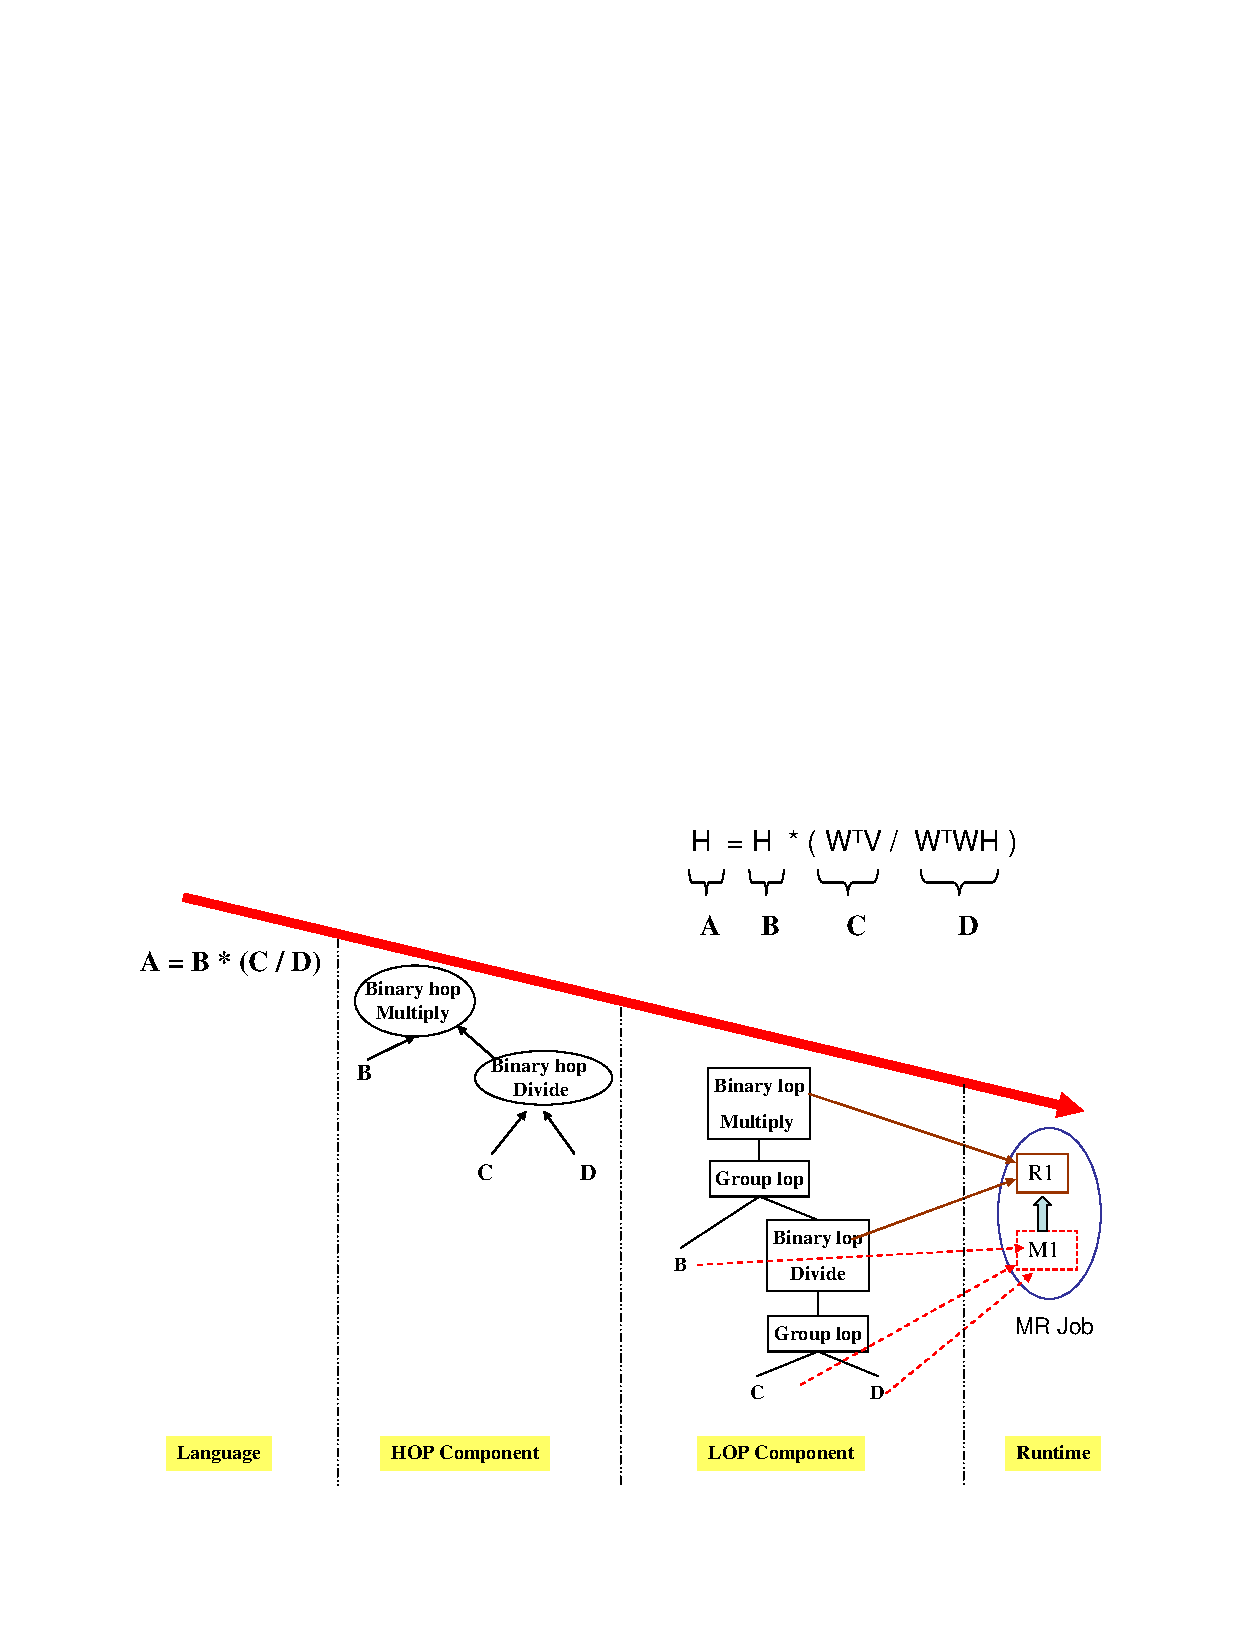
\includegraphics[width=3.75in]{example}
\end{tabular}
\caption{(a) Cost model for row-partitioning. We measure I/O cost and shuffle
cost separately. (b) Illustrating submatrix partitioning. The grey portion
corresponds to $A$, yellow corresponds to $B$, blue corresponds to $C$ and the
red portion corresponds to the $D$ matrix. (c) When the partitioning boundary
aligns with the block boundaries. Each small rectange indicates a block. 
(d) Case when the block boundaries do not align
with the partition boundary.}
\label{fig:costmodel}
\end{figure}

\eat{
\begin{figure*}
\begin{tabular}{|c|c|c|c|c|}
\hline
Method & I/O (c) & I/O (b) & Shuffle (c) & Shuffle (b) \\
\hline
Reblock & $\frac{mn}{rc} + 2m + mk$ & $8mn(k+3)$ & $m(\frac{n}{c} + k)$ &
$8mn(1+k)$ \\
\hline
Hashmap & $\frac{mn}{rc}(1 + rk)$ & $8mn(k+1) + 4mkM$ & 0 & 0\\
\hline
Join & $\frac{mn}{rc}(1 + rk)$ & $8mn(k+1) + 4mk$ & $\frac{mn}{c}$ &
$8mn + 4mk$ \\
\hline
\end{tabular}
\end{figure*}}


\subsection{Submatrix partitioning algorithms}
\label{sec:submatrix}
Now we discuss different ways to partition the input matrix into submatrices. As
mentioned in Section~\ref{sec:cvbackground}, this form of cross-validation is used for
unsupervised models such as PCA, SVD and NMF. Arbitrarily partitioning the
matrix using $2\times 2$ holdouts requires us to keep track of the columns and
rows corresponding to the different output matrices.
Since this is expensive for a large matrix, we develop a
two steps process: in the first step, we randomly shuffle the rows and columns
of the matrix, and following this we partition the matrix assuming contiguous
partitions. In this way, we only need to remember the indexes of the separators
between the output matrices. We describe both the steps in detail next.

\topicnoul{Shuffling:} In this step, we need to shuffle the rows and columns of the
matrix. To solve this, we use algorithm similar to join-based partitioning
for rows. In the pre-processing step, we randomly pick new row (column) indexes
for existing rows (columns) and populate a hash table. Subsequently, we join
this with the input dataset to create a randomly shuffled matrix. For this, we
use the hashmap based Map-side join since the number of entries in the idtable
is small (\#rows + \#columns). Note that this method is efficient since we are
only shuffling the non-zero entries in the matrix. The output of the shuffling
step is a matrix in cell format and may be subsequently blocked using a reblocking
step.

\topicnoul{Partitioning:} After the shuffling step, we partition the matrix into
contiguous boundaries. We use the example of $3\times 3$ Gabriel holdouts on a
$10\times 10$ matrix as shown in Figure~\ref{fig:costmodel}(b). Of the $9$ folds
that are generated, the figure shows the fold in which columns $4,5,6,7$ and
rows $4,5,6,7$ are held out and the rest are held in. For each cell in the input
matrix, we determine (1) the output matrix to which it belongs and (2) its index
in the output matrix. For instance, the cell $P_1 = (5,8)$ in the original
matrix belongs to the output matrix $B$. Its index in $B$ is $(1,4)$ since we
need to include all the yellow entries in $B$. Similarly, the cell $P_2 = (8,8)$
in the original matrix belongs to $D$ and its index in $D$ is $(4,4)$. Also, the
cell $P_3$ belongs to the matrix $A$ and its index in $A$ is $(2,1)$. 
The above algorithm requires us to iterate over every cell in the original matrix. 
If the input matrix is in block format, then we can instead iterate over the blocks in
the matrix, which is much more efficient.
If the partition boundary aligns with the block boundary (See
Figure~\ref{fig:costmodel}(c)), then we
can directly iterate over each block and return blocks as output (by computing
the correct block id $(b_i, b_j)$ for each input block).
If the partition boundary does not align with
the block boundary, then we cannot iterate over blocks. This is because in the
output matrices, the first column will be a partial block. 
In Figure~\ref{fig:costmodel}(d), the blocks indicated in red are partial, and
these correspond to the first row and column in the output matrices.
We currently provide two ways to handle this case: 
The first option is to iterate over the cells in
the block and use the cell-based approach. However, this is expensive as
previously indicated. The second option is to {\em nudge} the
partition boundaries such that they align with the block boundaries. Then, we
can direcly iterate over blocks and it is much faster. For example, in
Figure~\ref{fig:costmodel}(d), we move the partition boundaries (to the right
and below) such that it matches that of Figure~\ref{fig:costmodel}(c).
In large matrices, the difference in the size of the matrices obtained using this heuristic is very
minimal. For instance, consider a large matrix with size 101,000 rows by 101,000
columns and $1000 \times 1000$ block size. If we are interested to do $2\times
2$ Gabriel partitioning of the matrix, then all the four matrices need to be of
size $50,500 \times 50,500$. However, using the heuristic, we get four matrices of
size $50,000 \times 50,000$, $50,000\times 51,000$ and $51,000 \times 51,000$.
Such small differences in the sizes of the matrices do not bias the CV errors as
we experimentally observed on real-world topic modeling datasets~\cite{nips2010}.

\subsection{Cell-partitioning algorithms}
Now, we discuss algorithms for constructing folds by partitioning the cells of
the matrix. In this case, we only support holdout cross-validation, i.e., we
randomly holdout a small fraction of the cells in the matrix. As described
earlier, we explicitly store only the non-zero elements in the matrix. Hence,
iterating over the cells of the matrix does not uniformly partition the matrix.
Instead we generate bit matrices corresponding to the held out portion of the
matrix. Each bit matrix $B$ has entries either $0$ or $1$. If $B_{ij} = 1$, then
the corresponding entry in the data matrix $A$ is held out (i.e., test
component), other wise, the entry is held in (i.e., in the train component).
Note that the training algorithm (cvtrain) using cell-based partitioning needs
to be written based on these bit matrices. In fact, Kanagal et
al.~\cite{nips2010}
develop efficient strategies to learn {\em weighted NMF} models using such bit
matrices.


\eat{
\subsection{Sampling}
\label{sec:sampling}
In this section, we discuss algorithms for the different sampling techniques
required for implementing ensemble learning. We start with a discussion of
sampling with replacement. Then, we focus on weighted sampling.

\topic{Bootstrap sample: Sampling with Replacement} \\
We use a join-based approach for executing sampling with replacement, as
illustrated in the following example. Suppose we have an input data set $D$. with $n$
rows. To obtain a new sampled data set with $n$ rows (may include repeated
rows), we first sample $n$ numbers, each in $(1,n)$ and populate a relation $S$.
Next, we join $S$ with $D$ and obtain the sample. To construct multiple such
data sets, we generate multiple relations and join each of them with $D$.

\topic{Sampling with replacement from weighted samples} \\
For implementing AdaBoost, we need to sample a data set from a set of weighted
data points in each iteration. We discuss two approaches to solve this problem,
based on the previously proposed join approach. In the first method, we assume
that the set of weights corresponding to the tuples can fit in the memory of a
single machine. In this case, we construct the {\em cumulative distribution
function} (CDF) corresponding to the weights and build the relation $S$ using
the CDF. Following this, we use the previously proposed join mechanism for
building the sample. In the second approach, we construct $S$ using 
MapReduce jobs since the weights cannot be stored in memory. Suppose that each
data point has weight $w_i$ (and the sum of the weights is $W$). Also, suppose
that the number of mappers is $M$. In this case, our first job splits the input
into $M$ groups such that the sum of the weights in each group is $\frac{W}{M}$.
We choose each group such that it fits in memory. In the next job, we execute
weighted sampling on each group individually and compute the relation $S$.
Subsequently, we use the join job to compute the sample.
}

\subsection{Optimization}
\label{sec:optimization}

In this section, we discuss some of the optimization techniques that we have
developed, specifically for CV. As we illustration in
Section~\ref{sec:rowpartitioning}, there are three possible implementations of
row-partitioning. We show by analyzing the cost model that matrix
characteristics typically dictate the best method to use and discuss how to
choose the best possible plan. After this we discuss some other optimizations
that we developed in SystemML.

\topic{Selecting plans for partitioning}
\topicnoul{Cost Model:} The costs for the three algorithms described above is
shown in Figure~\ref{fig:costmodel}. We measure the costs for I/O and shuffling in
terms of two parameters: First, the number of key-value pairs and second, the
total number of bytes. As we can see from the table, there is no clear winner
among the three approaches. The hash map approach has $0$ shuffle cost since it
is a Map-only job. However, it has a significant I/O cost since the map table
needs to be read by each of the mappers. Similarly, the join approach has a
small amount of shuffle cost, but its I/O cost exceeds that of the Reblock job
(in terms of the number of key-value pairs). 
%Another important factor that
%denotes the efficiency is the type of the output generated by the partitioning.
%In SystemML, before executing
%an operation (say matrix multiplication or addition), both the input matrices
%need to have the same block size.
%As output of the reblock job, we get $1000\times 1000$ blocks (since we can
%cache rows and reblock the rows at the reducer). Hence, we can directly use the
%output of partitioning for further operations. However, with the join-based
%methods, we get partial rows

\topicnoul{Row-partitioning:}
The
hashmap technique has zero shuffle cost, but its I/O cost is very high. Further,
it is limited by the size of the memory in each mapper. Join-based partitioning
has low shuffle cost, but its I/O cost is more than that of reblock-based
method. We currently use a simple heuristic to pick the method to use.
Initially, we check the number of rows $m$ in the matrix. If $4mk$ bytes fit in
the memory of each mapper, then we use the hash map based strategy. Otherwise,
we compute the shuffle costs for the reblock and the join jobs and select the
method with the smaller shuffle cost. If they are comparable in the shuffle cost
we use the method with the smaller I/O cost.

\topicnoul{Submatrix-partitioning:}
Tian et al.~\cite{DBLP:conf/icde/TianK11} and Kang et al.~\cite{DBLP:conf/icdm/KangTF09} illustrate
the benefits of using blocking for representing large matrices efficiently.
Instead of maintaining key value pairs for each entry in the matrix, it is more
efficient to maintain key value pairs for blocks in the matrix. With respect to
partitioning, blocking is even more beneficial. Note that most of the data
provided by users is in cell format (i,j,v) since it is standard across
different applications and is easy to parse.
Suppose that we want to do
sub-matrix partitioning of an input matrix in cell format. Then, we can use one
of two methods. In the first method, we use the cell-based algorithm to execute
the partitioning. Note that in the shuffle phase, we are replicating each cell
$hl$ times. The number of key value pairs in the shuffle stage is $hlmn$. In the
second method we first use the reblock job to block the matrix and then use the
algorithm to partition and replicate blocks in the matrix. The number of key
value pairs in the shuffle stage is $\frac{hlmn}{rc}$. Note that even though we
are making two passes over the data, the second method may be faster whenever
the shuffle stage is the bottleneck.

\topic{Other optimization}
\begin{enumerate}
\item {Replication ({\em concat}):}
The algorithms for partitioning that we have described so far construct all the
folds at the end of the partitioning step. Note that we replicate the dataset for
each fold. However, we may not have space to construct all the folds in the
beginning, especially when we are interested in very large-scale 10000-fold
cross-validation. For this case, we support alternative plans in which we first
evaluate the partitions in the first job. Subsequently, we combine the
partitions to generate folds. For this, we introduce the {\em concat} construct
in SystemML. {\tt concat(A,B,`row')} concatenates the rows of matrices {\tt A}
($m\times n$) and {\tt B} ($p\times n$) to get a new matrix {\tt C}
$((m+p)\times n)$. Similarly, we also support {\tt concat(X,Y,`col')}. For
$3\times 3$ sub-matrix partitioning (Section~\ref{sec:submatrix}), we first
generate the $9$ matrices $\{X_1, X_2, \dots X_9\}$ shown in
Figure~\ref{fig:costmodel}(b) and then use {\tt concat($X_4$, $X_6$,`col')} to
generate the $B$ matrix.

\item {Piggybacking:}
To partition the matrix column wise, we can use the row-based partitioning
algorithms described earlier. However we need to transpose the matrix first for
this purpose. In SystemML, several low-level operations are grouped together in
a given MapReduce job to efficiently execute the operations by making fewer
passes over the data. Here, we allow the transpose operation (and other unary
operators) to be executed within the map-phase of the partitioning jobs.

\item {Random sampling:} Ocassionally, random sampling may not be necessary to
construct folds for $k$-fold CV. For this case, we directly use the Map-side
join approach. We do not need to construct the hash map for this case, rather we
can simply use rowid \% number of folds.
\end{enumerate}


\subsection{Scheduling}
After compiling the DML program, we obtain a MapReduce dag, which we need to
schedule over the cluster. For the CV construct, we obtain a disconnected dag
with as many components as the number of folds (since each fold is independent
of the other folds). While we postpone the scheduling of arbitrary MapReduce dags to
future work, we focus on scheduling the tasks, based on the resources available
at hand. We abstract each component in our dag to comprise of two
tasks: first, {\em fold construction}, and second, {\em error
computation}.  There are several different ways of scheduling the tasks: As mentioned
earlier, we could generate all folds at once, or we could exploit the {\em
concat} operator to generate folds one-by-one. In fact, based on the amount of
storage available on the HDFS, we can generate as many folds as feasible.
Similarly, we can simultaneously compute the errors for arbitrary number of
folds, based on the amount of compute servers available at any time. We perform
a preliminary experimental analysis for scheduling and report on the results in
Section~\ref{sec:experiment}.

\section{Implementation Details}
\label{sec:implementation}
In SystemML, we implement cross-validation as a high level language construct,
rather than a user-defined function. This choice is motivated by the
scalability: to support generic cross-validation via UDFs requires
implementation of arbitrary functions which cannot be optimized effectively. On
the other hand, since we know the exact semantics for CV (i.e., fold
construction, multiple learning and evaluation), we can effectively parallelize
and schedule the computation as necessary. As discussed in
Section~\ref{sec:background}, SystemML is implemented using a four layer
abstraction. To incorporate the CV language constructs, we implement parsing
and introduce additional hops and lops as required. For creating multiple
outputs for partitioning, we use the {\tt MultipleOuputs} module in Hadoop
0.20.1. In this section we discuss two key issues that we faced while compiling
the construct.

\topic{Compilation Issues}\\
In addition to compiling the main program containing the CV statement, we need to
additionally compile and validate the two functions cvtrain and cvtest.
Currently, SystemML statically checks the validity of each line in the program,
for example, whether matrix multiplication $C = A\times B$ is legal. However, we
will not have the sizes of the matrices at compile time since our
partitioning step uses random sampling techniques. Further the sizes of the
matrices are used for optimizing the program. For example, SystemML uses the
size of the inner dimension to decide whether to use CPMM or RMM for matrix
multiplications~\cite{DBLP:conf/icde/TianK11}. Hence, we propose two 
strategies for compiling DML programs.

\begin{enumerate}
\item{\underline{Runtime compilation:}}
We can compile the train and test programs at runtime, for each fold after
obtaining the sizes of the matrices resulting from the partitioning step. The
disadvantage is that we are compiling as many times as there are folds. However,
we are guaranteed to pick the most optimal plan for each fold.
\item{\uline{Incremental compilation with additional checking at runtime:}}
The other strategy that we adopt is to compute the plan at compile time itself
by assuming expected values for the unknown parameters of the matrices. We use
techniques from type inference~\cite{} for verifying the validity of the
programs as much as possible during compile time and postpone the complete
checking to runtime. Although we only compile the whole program once, we cannot
exploit the optimization machinery to the fullest extent.
\end{enumerate}

Since the bulk of the time taken is for executing the testing and the training
routines, and the time taken for compilation is very small, we adopt the runtime
compilation approach.


\topic{Pseudo random sampling on Hadoop}\\
SystemML uses random sampling to compute the various folds for cross-validation.
Since SystemML is based on Hadoop, which is a parallel computing framework, we
need to ensure that the random sampling is unbiased and perfectly pseudo random.
For this purpose, we use {\tt WELL1024}~\cite{L'Ecuyer:1990:RNS:84537.84555}, a
long period random number generator (PRNG). WELL1024 provides a PRNG with period
approximately, $2^{1000}$. Further, it splits the entire period into $2^{300}$
streams, each of length $2^{700}$. Each of these streams are further partitioned
into $2^{300}$ substreams, each of size $2^{400}$.  It provides routines to {\em
skip} over substreams and jump to the next substream.  Now we describe how we
incorporate the WELL1024 PRNG into SystemML for partitioning large datasets.
Each mapper requires a particular number of substreams based on the type of
partitioning required. For each mapper, we compute its unique identifier and
assign the corresponding streams. For example, suppose that each mapper requires
2 streams (k-fold stratified cv with domain size = 2). In that case, if we get
to the mapper with id = 4, we first skip 6 times to get the first stream for the
mapper and skip again to get the second stream for the mapper. The time taken
for skipping over substreams is very small. Experimental results reveal that
skipping over a 10,000 substreams requires less than a second.

 \topic{Supporting Stratification} \\
As mentioned in Section~\ref{sec:background}, supervised learning tasks require
the folds to be stratified -- based on the class label. We support
stratification for row-based partitioning tasks using multiple seeds. We
illustrate with an example. Suppose that we want to classify emails as spam or
genuine. In this case, we use $2$ seeds, one for each email type. For each row,
we examine its class label and sample from the appropriate seed.


\section{Experimental Evaluation}
\label{sec:experiment}

We start with a description of the experimental setup and the main objectives
of our analysis.

\subsection{Objectives}
The main objectives of our experimental analysis are as follows.
\begin{enumerate}
\item {\em Necessity of a declarative system for large-scale meta-learning:}
Here, we compare the performance of the proposed algorithms for row partitioning
for various matrix characteristics.
\item {\em Scale-up of partitioning jobs:} Here, we demonstrate the {\em
scale-up} and {\em speed-up} of the partitioning jobs for rows and sub-matrices.
\item {\em Illustrating advantages of optimization \& scheduling}
\end{enumerate}

\subsection{Results}
\topic{Necessity of a declarative system for large-scale machine learning} \\
We consider different matrix characteristics $C_1$, $C_2$ and $C_3$ as defined
below and execute different algorithms for row partitioning over them
(Section~\ref{sec:design}). We denote $P_1$ to be the method using
reblock. $P_2$ is the method using hashmap and $P_3$ to be the method using
joins.
\begin{enumerate}
\item $C_1$: {\em Number of rows:} For small number of rows, we see that $P_2$
is the best method since the hash map fits in memory. As we increase the number
of rows, the reblock method wins since we cannot maintain hashmap in memory. 
When we increase the number of rows further, the join method ultimately beats
out the remaining methods. Note that this is in spite of join method using both
map and reduce phases.
\item $C_2$: {\em Number of columns} Here, we plot the performance of our row
partitioning algorithms over matrices with different number of columns. As we
can see from the plots, when the number of columns is low, the reblock method
works well. However, when the number of columns is very large, the row block may
not fit in memory and the join method works well.
\item $C_3$ {\em Number of non-zeros} Here, we fix the number of rows and
columns in the matrix and gradually increase the number of non-zero elements in
the matrix. As expected, we find that its behavior is similar to increase the
number of columns in the matrix.
\end{enumerate}

As shown by the above figures, there is no clear winner among the three methods
and the matrix characteristics dictate the best approach for partitioning. Given
the large number of factors involved, a declarative system is essential for
scaling large-scale cross-validation and ensemble learning tasks.

\topic{Scalability of partitioning jobs:} \\
Here, we demonstrate the scale-up and speed-up of the partitioning
algorithms. We run the following experiments.

\begin{enumerate}
\item {\em Speed-up:} We carry out two experiments here. In the first
experiment, we increase the number of mappers and measure the total speedup
obtained for the row partitioning and the matrix partitioning algorithms. In the
second experiment, we increase both the number of mappers and reducers and
measure the speedup obtained. We notice here that the speedup in the second
experiment is almost equal to the speedup obtianed in the first experiment. This
is because the number of reducers actually used by Hadoop is equal to the number
of files written (e.g., for $k$-fold cross-validation it is $2k$).

\item {\em Scale-up:} Here, we carry out the following experiments. In the first
experiment, we increase the number of rows and simultaneously increase the
number of mappers \& reducers to measure the time taken for row-based k-fold
cross-validation. Next, we repeat the experiment by increasing the column size
of the matrix. Following this, we execute the above experiments for the case of
sub-matrix partitioning.

\item {\em Increasing number of folds} We carry out two experiments here. In the
first experiment, we execute row-based k-fold cross-validation with different values of
$k = 5, 10, 15$. As shown in Figure~\ref{fig:results}(f), as we increase the
number of folds, the amount of time taken increases linearly.

\item {\em Submatrix scalability} In this experiment, we measure the scalability
of the submatrix partitioning jobs. In Figure~\ref{fig:results}(g), we measure
the scalability of the cell-based partitioning jobs. As we increase the number
of rows in the matrix, we obtain a close to linear increase the computation
time. However, the slope is dependent on the number of columns in the matrix. In
Figure~\ref{fig:results}(h), we perform the same experiment on the block-based
partitioning job and obtain similar results.
\end{enumerate}


\begin{figure*}
\begin{tabular}{ccc}
%\includegraphics[width=2.5in]{time.pdf} &
%\includegraphics[width=2.5in]{time2.pdf} &
%\includegraphics[width=2.5in]{kfold.pdf} \\
%(a) & (b) Row partitioning & (c) Linearly increases in $k$ \\

\begin{minipage}{2.3in}
\begin{tabular}{|c|ccc|}
\hline
&Reblock& Hashmap& Join \\
\hline
Case 1 &&&\\
Case 2 &&&\\
Case 3 &&&\\
Case 4 &&&\\
Case 5 &&&\\
\hline
\end{tabular}
\end{minipage} &
\hspace*{-0.2in}
\begin{minipage}{2.3in}
\includegraphics[angle=-90,width=2.3in]{blank.pdf}
\end{minipage} &
\hspace*{-0.2in}
\begin{minipage}{2.3in}
\includegraphics[angle=-90,width=2.3in]{blank.pdf}
\end{minipage} \\
(a) Declarative & (b) Scaleup (Row) & (c) Scaleup (Row) \\

\includegraphics[angle=-90,width=2.3in]{blank.pdf} &
\hspace*{-0.2in}
\includegraphics[angle=-90,width=2.3in]{blank.pdf} &
\hspace*{-0.2in}
\includegraphics[angle=-90,width=2.3in]{kfold.pdf} \\
(d) Speedup (Row) & (e) Speedup (Row) & (f) Scalability (folds) \\


\includegraphics[angle=-90,width=2.3in]{submatrix-cell.pdf} &
\hspace*{-0.2in}
\includegraphics[angle=-90,width=2.3in]{all-block.pdf} &
\hspace*{-0.2in}
\includegraphics[angle=-90,width=2.3in]{optimization.pdf} \\
(g) Scalability Submatrix (cell) & (h) Scalability Submatrix (block) & (i) Optimization \\


\includegraphics[angle=-90,width=2.3in]{blank.pdf} &
\hspace*{-0.2in}
\includegraphics[angle=-90,width=2.3in]{blank.pdf} &
\hspace*{-0.2in}
\includegraphics[angle=-90,width=2.3in]{blank.pdf} \\
(j) Scheduling (concat) & (k) Scalability CV (NMF) & (l) Scalability CV (LR) \\

\end{tabular}

\caption{Experimental Results}
\label{fig:results}
\end{figure*}

\topic{Optimization}

\begin{itemize}
\item {\em Blocking for submatrix partitioning:} 
In this experiment, we illustrate the advantages of
blocking the input matrix for submatrix partitioning. We start with a matrix in
cell format and partition it using two different plans. In the first plan $P_1$, we
execute $2\times 2$ partitioning using the cell-based approach
(Section~\ref{sec:}. In the second plan $P_2$, we use a two step process in which we 
initially block the matrix using a reblock job and subsequently use the
block approach for partitioning. We measure the time taken for each case. For
the second case, we compute the time taken for both the reblocking and the
partitioning. The results are shown in Figure~\ref{fig:results}(i). We execute
two experiments with different column sizes. In each experiment, we vary the
number of rows in the matrix.
As shown in the figure, the time taken in $P_2$ is much less than $P_1$. We
would like to note here that this may seem counter intuitive
since we are actually making two passes over the data. The reason for this is
that in the first case, we are replicating cells (while shuffling) where as in
the second case we are only replicating blocks, which are much fewer in number.
\end{itemize}


\topic{\em Scheduling:}\\ This allows us to replace the partition operator
with multiple concat operators, essentially creating a HOPS/LOPS dag which is
disconnected. This allows us to start training on the 1st fold, while the second
fold is being constructed. Note that this scheduling must be aware of the amount
of disk space that is available on the HDFS. While learning, we consume the
folds and can create additional space for subsequent folds. I am planning to
test the three approaches (measure make-span: time for entire task to complete)
\begin{enumerate}
\item Construct all folds at once. The graph will essentially show that for
$k=10$ and above, Hadoop will throw I/O errors due to lack of space. Space is
the biggest constraint for large-scale.
\item One-by-one: This is the other extreme when we learn the fold, then build
the next fold and so on.
\item Our scheduling: Intelligently schedule jobs by making use of available
resources.
\end{enumerate}

\eat{
\begin{figure}
\centering
\begin{tabular}{cc}
\end{tabular}
\caption{
In (e), the time taken for row partitioning increases as $k$ increases. This is because
we are currently replicating the dataset. We need to avoid copying over the dataset
multiple times.}
\end{figure}
}

\section{Conclusions}

Massive amounts of data generated on the web are used to routinely train very
complex machine learning models for solving a range of problems such as spam
detection, recommender systems, personalized search and advertising;
Consequently, verifying the quality of machine learned models has become an
important task. Cross-validation is a versatile tool that has been extensively
used for solving this problem, as well as a number of related problems such as
model-selection and feature selection. In this paper, we build a system that
provides the ability to cross-validate all possible machine learning models
(including unsupervised models) over very large-scale datasets using the
MapReduce framework. As we show in the paper, owing to the multitude of methods
to cross-validate a given machine learning model (for e.g., partitioning
techniques) and the various potential implementation strategies, we need to
develop a declarative system that can choose the best possible plan for a given
cross-validation task.  In future, we intend to extend our system for performing
other meta-learning tasks such as boosting, stacking and other ensemble
strategies. We also plan to develop scalable cross-validation strategies for non
i.i.d samples such as relational learning models.

\section{Related work}
\label{sec:related}
\topic{Large-scale machine learning:}
Large-scale machine learning has become an important research task given the
{\em application pull} -- spam detection, personalized search, recommendation
application and so on and {\em technology push} -- availability of large-scale data processing
tools such as MapReduce and multicore systems. There have been a number of
systems built Apache Mahout~\cite{mahout}, Google prediction API~\cite{gapi},
SystemML~\cite{DBLP:conf/icde/TianK11}, GraphLab~\cite{Low+al:uai10graphlab},
Pegasus~\cite{DBLP:conf/icdm/KangTF09}. Further, there has been a
lot of literature including Chu et al.~\cite{DBLP:conf/nips/ChuKLYBNO06}, Cohen
et al.~\cite{DBLP:journals/pvldb/CohenDDHW09}. Our work
is largely an extension to such large scale machine learning systems;
specifically, we extend SystemML to support cross-validation as a first class
citizen.

\topic{Meta-learning:}
Meta-learning is an area of machine learning where models are trained over
meta-data of the machine learning experiments. Broadly, this includes
cross-validation algorithms and {\em ensemble learning} algorithms such as {\em
Boosting}~\cite{DBLP:journals/jcss/FreundS97}, {\em
Bagging}~\cite{springerlink:10.1007/BF00058655}, {\em
Stacking}~\cite{DBLP:journals/scholarpedia/Polikar09} and so on.
Ensembles were extensively used in the recently concluded Netflix
challenge to improve recommendation accuracies. In
recent work, Panda et al.~\cite{DBLP:journals/pvldb/PandaHBB09} describe PLANET, a system
developed at Google, for building ensembles with the {\em decision tree} model
over very large scale data over MapReduce. In this work, as opposed to PLANET, we are developing a
declarative system for generic meta learning for all kinds of models. In
addition, we have developed efficient techniques for sampling with replacement on
MapReduce, using which we plan to exploit the full potential of Bagging and
other algorithms.

\bibliographystyle{abbrv}
{
\small
\bibliography{internreport}}

\appendix





\section{Cost model -- Details}
Assume an $m \times n$ matrix with $r\times c$ blocks. Assume a $k$-fold
cross-validation. In the worst case, there are 8 bytes for each entry in the
block. Also suppose that the number of mappers used is $M$.

\topicnoul{Using reblock:}
In this case, we need to use 2 jobs: In the first job, we compute the row-blocks
and in the second job, we execute partitioning and replication. For the first
job,
\begin{enumerate}
\item I-cost: $\frac{mn}{rc}$ blocks, ($8mn$ bytes)
\item Shuffle-cost: $\frac{mn}{c}$ blocks, ($8mn$ bytes)
\item O-cost: $m$ blocks, ($8mn$ bytes)
\end{enumerate}

\noindent For the second job,
\begin{enumerate}
\item I-cost: $m$ blocks, $8mn$ bytes
\item Shuffle-cost: $mk$ blocks, $8kmn$ bytes
\item O-cost: $mk$ blocks, $8kmn$ bytes
\end{enumerate}

\noindent Note that when using reblock, we can use at most $2k$ reducers because
the domain of the reducer key is just $2k$.

\topicnoul{Using hashmap:}
In this case, a  map-only job will suffice since we already know the new row-ids
for each input row in the matrix. The costs in this case are:

\begin{enumerate}
\item I-cost: $\frac{mn}{rc}$ blocks for matrix, $mkM$ for hash map. Note that
hash maps need to be read once for each mapper ($8mn + 4mkM$ bytes)
\item Shuffle-cost: 0
\item O-cost: $\frac{mnk}{c}$ blocks ($8mnk$ bytes)
\end{enumerate}

\topicnoul{Using Joins:}
\begin{enumerate}
\item I-cost: $\frac{mn}{rc}$ blocks for matrix, $mk$ for sample table. $(8mn +
4mk)$
\item Shuffle-cost: $\frac{mn}{c}$ for matrix, $mk$ for sample table. $(8mn +
4mk)$
\item O-cost: $\frac{mnk}{c}$ blocks ($8mnk$ bytes)
\end{enumerate}


\eat{
\topic{Cost model} \\
Assume an $m\times n$ matrix with $r\times c$ block size. We compute the number
of key-value pairs emitted and the state maintained by the mapper and reducer
phases.
\hspace*{-0.3in}
}

\section{Things to do}
As per last discussion, we will focus on efficiently implementing
cross-validation completely. In order to finish this, we will require:
\subsection{Implementation}
During the internship, I implemented the row-based partitioning. It was usually
preceeded by reblocking which created the row-blocks. However, we need the
following algorithms for the experiments: hashmap-based partitioning and
join-based partitioning. As a pre-processing step, we need to compute the sample
tables for each of the input rows in the matrix. For example, in the case of
k-fold cross-validation, for each row of the input matrix, we need to determine
its new rowid in each of the output matrices to which it belongs. This operation
can be implemented as a control module itself.

\begin{enumerate}
\item {\em Hashmap-based partitioning:} 
In the configure() step, we need to load the hashmap into memory. In the map()
routine, (1) for each block, we cut it into rows (2) for each row in the block,
we determine the rowid and partition id from the hashmap (3) Output it to the
relevant file using MultipleOutputs.
\item {\em Join-based partitioning:}
Here, we use the standard {\em reduce-side join} for executing the join-based
partitioning.
\end{enumerate}

\topicnoul{CV for Linear/Incremental models:}
In our effort to provide a generic framework for executing CV over all
possible machine learning models, we lose the advantages of executing specific
CV algorithms. For instance, we can cross-validate linear regression
models using parametric methods~\cite{survey} by only making a single pass over the
data set. Similarly, we can cross-validate SVM
models~\cite{DBLP:conf/nips/CauwenberghsP00} efficiently by exploiting the
incremental algorithms for learning/un-learning such models. These optimization
tricks are specific to each model. To support such optimization, we currently
support an alternative implementation of CV in which we first partition the data
set into components. Then we train a model on each component. Incremental models
typically 


allow the user to specify the following information

\begin{enumerate}
\item that the training algorithm is incremental via a hint
and the associated routines to combine partial models 
\end{enumerate}



Computing sufficient statistics by
training portions of each model and using the additive property.
Piggy back the learning onto the mapper.


\end{document}
